\section{Задание}

Нахожу радиус и цент окружности по теореме Гершгорина, в итоге получаю области для 
собственных значений:

\begin{figure}[H]
    \centering
    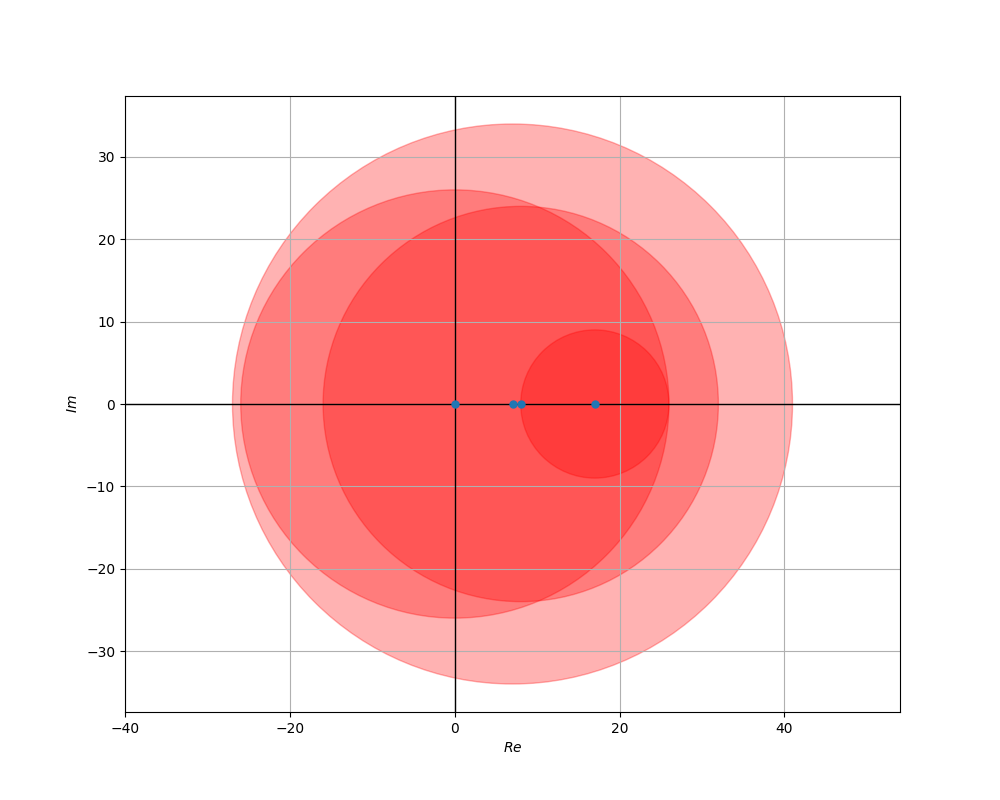
\includegraphics[trim={0 0 0 0},clip,width=\textwidth]{Imgs/evs.png}
    \label{evs}
\end{figure}

Вспомним что собственные значени для транспонированной матрици равны 
поэтому получим второе ограничение:

\begin{figure}[H]
    \centering
    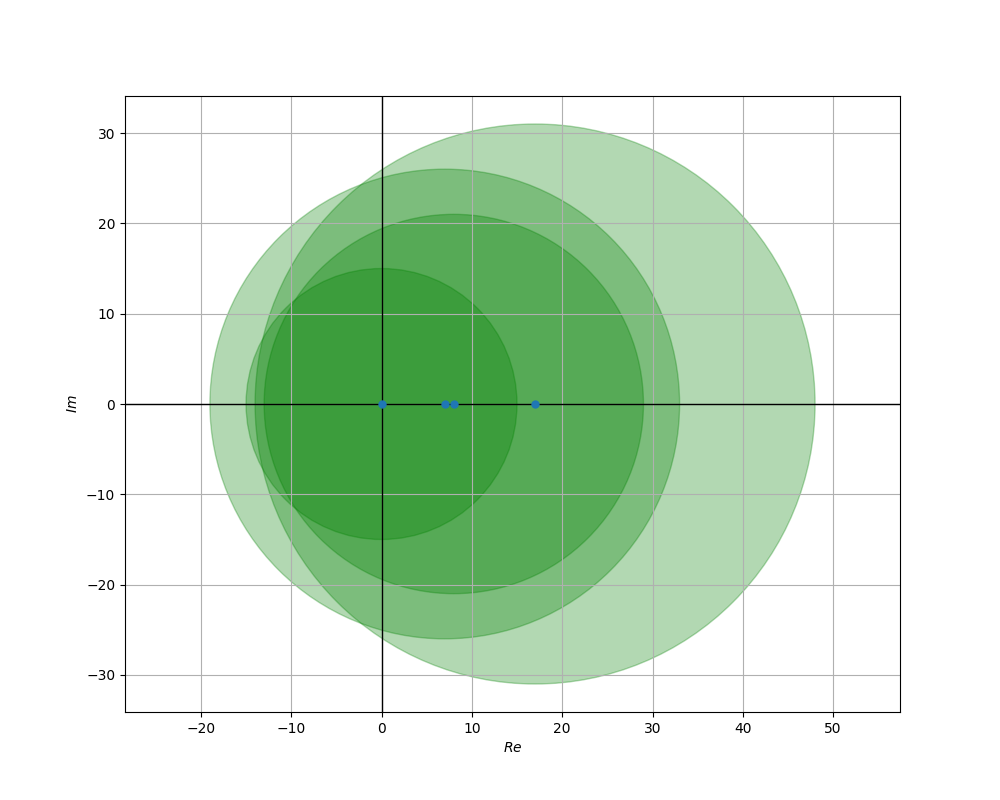
\includegraphics[trim={0 0 0 0},clip,width=\textwidth]{Imgs/evs_t.png}
    \label{evs_t}
\end{figure}

Обединение этих картин дает мне:

\begin{figure}[H]
    \centering
    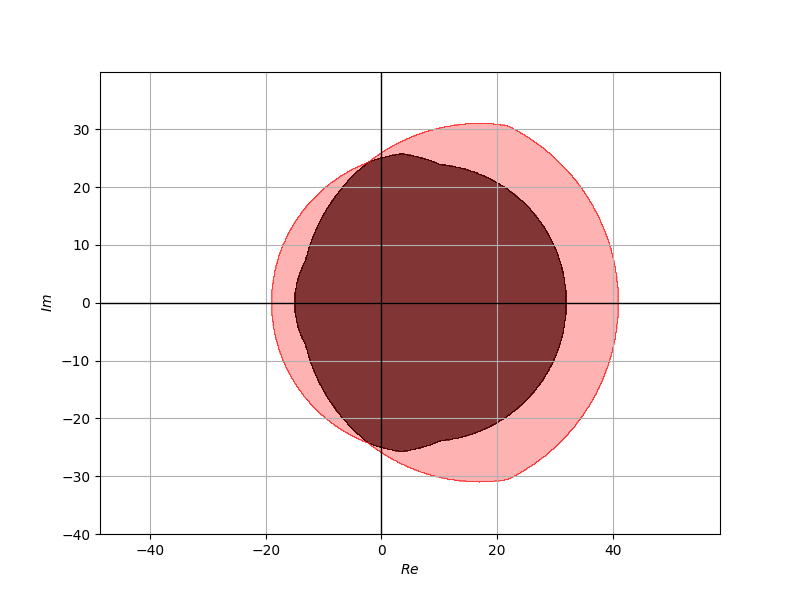
\includegraphics[trim={0 0 0 0},clip,width=\textwidth]{Imgs/bool_and.png}
    \label{and}
\end{figure}

Но так как собственные значени встречаются попарно поэтому получим, что там где 
есть тольк одно собственное число, там число может лежать только на оси $X$, такая область
отмкчена фиолетовым. В красной области собственне числа могут существовать где угодно (не только на оси),
но все еще в нутри собственных кругов отмеченных зеленым.



